The 95\% confidence level upper limits on the sV and sA model couplings, $\sqrtgqgX$, and the tS model coupling, $\gqX$, which are obtained from each of the \monoX channels, are presented in figs.~\ref{fig:results_sVsA_rat05} - \ref{fig:results_tS}. These quantities were evaluated as described in appendix \ref{Appendix_limitsetting} and correspond to the best limits of each signal region tested.

In each plot, the grey region represents the phase space where no meaningful limit was obtained, that is, where the limit of at least one of the couplings was found to be greater than $4\pi$ (and thus well out of the perturbative region). The white (hatched) regions coincide with those mass points which yield an initial (final) value of $\sqrtgqgX$ which fails to satisfy our requirement that $\Gamma < \Mmed / 2$. Note that only the \monojet channel produced limits which survive this requirement when $\gX / \gq$ = 0.2, as shown in fig. \ref{fig:results_sVsA_rat02}. We subsequently omit the plots containing the associated limits for the \monoZ and \monoWZ channels.

We note here that values of $\sqrtgqgX$ and $\gqX$ smaller than our hard upper limit of 4$\pi$, beyond which any results are considered meaningless, may also become increasingly invalid as they become less perturbative. Additionally, values for which the width is just within our upper validity bound of $\Mmed/2$ may be pushed over into the invalid range with the addition of new particles, not considered here, which would serve to increase the mediator width.

Large DM masses: small cross sections, limited by ATLAS analysis optimisation, requires more data or further optimisation. Small DM masses: have low $\met$, would require more statistics. (True for mono-Z and I assume monojet also.)

The results are discussed according to channel below.

\iffalse
\textcolor{magenta}{This section should include:}
\begin{enumerate}
\item \textcolor{magenta}{Plots for $\sigma(pp \rightarrow X \chi \bar{\chi}$ as a function of $\mX$ for fixed $\Mmed$ and $f$ along with the limits on $f$ using $\sigma \sim f^{4}$.}
\item \textcolor{magenta}{Brief interpretation of the results. I.e. explain "in words" what the plots illustrate.}
\item \textcolor{magenta}{Comparison with previous results (?).}
\end{enumerate}
\fi

\subsection{Mono-jet channel}

The upper limits on the coupling combination $\sqrtgqgX$ (calculated at 95\% confidence interval) of the sV and sA models, obtained in the \monojet channel, are displayed in the left-hand column of figs.~\ref{fig:results_sVsA_rat05, fig:results_sVsA_rat1, fig:results_sVsA_rat2, fig:results_sVsA_rat5}, for $g_q/\gX =$ 0.5, 1, 2 and 5 respectively. Additional results for the $g_q/\gX =$ 0.2 case are also shown separately in fig.~\ref{fig:results_sVsA_rat02}, as these limits are only meaningful within the \monojet channel.

Examining first the sV model, we see stronger limits in the region of phase space where $\Mmed > \mX$ (why?), and weaker limits where $\Mmed < \mX$ (due to small cross sections). The weakest limits result for large $\mX$ or large $\Mmed$, and in fact are so weak that they are pushed into the region of invalidity where $\Gamma > \Mmed/2$; this is because although the acceptance is considerably higher in these regions compared to low masses, the cross section is sufficiently small that this effect prevails. Within the valid region ($\mX \in [1, 100]$ GeV and $\Mmed \in [1, 200]$ GeV), the limit on $\sqrtgqgX$ generally ranges from 0.1 to 0.7, with a handful of on-shell masses reaching a limit of $\sim$0.05 in the large $\gX / \gq$ case.

As the ratio $\gX / \gq$ varies, the coupling limits tend to remain approximately constant, as is expected when the coupling (and hence the width) has been demonstrated to have little effect on kinematic behaviour (and using the assumptions of eq.~\ref{eq:sigma_propto_couplings_schan}). As the ratio increases, points in the region $\Mmed > \mX$ disappear as the initial condition, $\gq = 1$, leads to failure of the width condition. However, one could easily have chosen a smaller initial value of $\gq$ to recover these points, and we suggest that the limits in this region would be quite similar to those seen in the $\gX / \gq$ = 0.2 and 0.5 cases.

In the large ratio scenario, limits for $\mX = 1000$ GeV start to become valid. This is because if $\sqrtgqgX$ remains constant but the $\gX / \gq$ increases then the value of $\gq$ is pushed downward and so the width, which is dominated by decays to SM particles, decreases.

The uncertainties on the limits displayed here generally range from \comm{??}\% to \comm{??}\%, and are dominated by \comm{X}.

Moving next to the sA model within this channel, we find that the strongest limits are obtained when $\mX > \Mmed$, thanks to both an improved acceptance and a higher cross section. Similarly to the sV model, as the couplings ratio increases, the limit remains approximately constant, and the high $\mX$ points move back into the valid region. The uncertainties for this model are dominated by X and are within the range $X \sim Y$\%.

\subsection{Mono-$Z$ channel}

The simplicity of the \monoZ channel relative to the \monojet channel, and the speed of its production within \MG, allowed us to study a finer granularity of points in the mass phase space. The resulting limits on the sV and sA models are shown in the central column of figs.~\ref{fig:results_sVsA_rat05, fig:results_sVsA_rat1, fig:results_sVsA_rat2, fig:results_sVsA_rat5}. The behaviour of the limits as $\gX / \gq$ varies is similar to that within the \monojet channel, and overall the limits are weaker compared to that channel by a factor of a few.

The total relative uncertainties on $\sqrtgqgX$ are generally within 10\%, but can range up to 80\% in a few cases.

The advantage of the mono-boson channels is in the study of the tS model; since this was not included in the \monojet channel the strongest limits are obtained with the \monoZ analysis, and are shown in the left-hand side of fig.~\ref{fig:results_tS}. In general the tS model limits are weaker than the corresponding $s$-channel points (why?), note that the scale here is increased by a factor of 10. We find stronger limits for smaller $\mX$ and $\Mmed$ masses, where larger cross sections compensate for lower acceptances at these points.

\subsection{Mono-$W/Z$ channel}

The limits on the couplings of the sV, sA and tS models, obtained within the \monoWZ channel, are shown in the right-hand column of figs.~\ref{fig:results_sVsA_rat05, fig:results_sVsA_rat1, fig:results_sVsA_rat2, fig:results_sVsA_rat5, fig:results_tS}. This channel was studied to compare with the leptonic \monoZ channel in particular, but a coarser selection of masses was chosen as the limits were initially found to be somewhat weaker. Additionally, further estimates were made: a) as the kinematic behaviour is reasonable independent of the couplings, a single acceptance was found for each ($\mX$, $\Mmed$) combination and applied to each value of $\gX / \gq$, and b) complete systematic uncertainties were generated for a subset of masses and compared to those from the \monoZ channel; from this comparison the \monoZ systematic uncertainties were multiplied by 3 and then applied to the \monoWZ limits. As a result, the limits obtained in this channel are not intended to be rigorously testable; rather, they are used more to indicate qualitatively how the channel compares.

The ATLAS \monoWZ analysis was not optimised for a simplified model interpretation, and much of the phase space produced insignificant numbers of events passing the event selection, with up to 200 thousand events generated. Generally, the limits are a factor of a few weaker again than those from the \monoZ channel, which is both consistent with the limits on the EFT models studied in the ATLAS analyses, and expected following the use of a cut-and-count interpretation of the \monoWZ public results (can we say this? Point is to compare with them probably doing a shape analysis to improve their limits). Some exceptions do exist however - the low-$\Mmed$ region of the sA model shows limits comparable to those within the \monoZ channel.

Overall, the uncertainties from this channel lie within the range XXX.

\afterpage{\clearpage}

%\begin{figure}
%  \centering
%  \begin{subfigure}[t]{0.32\textwidth}
%    \centering
%    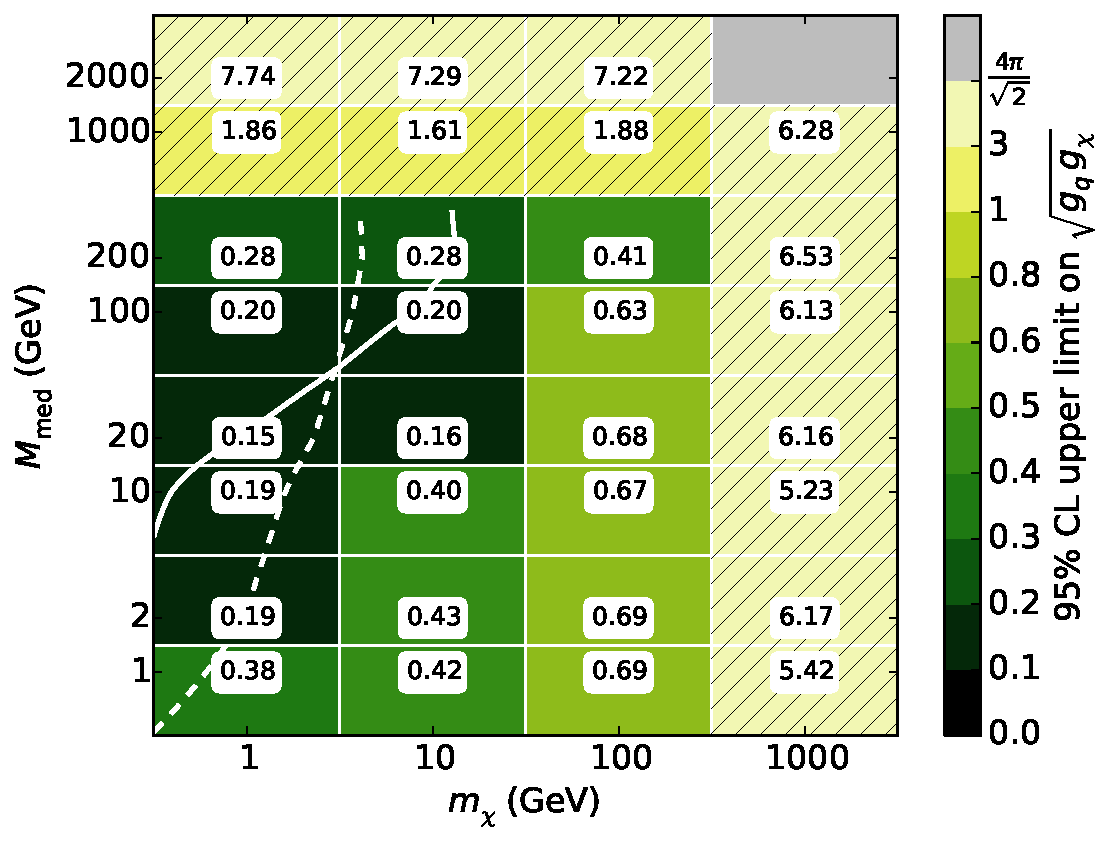
\includegraphics[width=1.\textwidth]{figures/grid_basepoints_SVD_rat05_monojet.pdf}
%    \caption{sV model, $g_q/g_{\chi} = 0.5$, \monojet channel.}
%  \end{subfigure}
%  \caption{}
%\end{figure}

\begin{sidewaysfigure}
  \centering
  \begin{subfigure}[t]{0.32\textwidth}
    \centering
    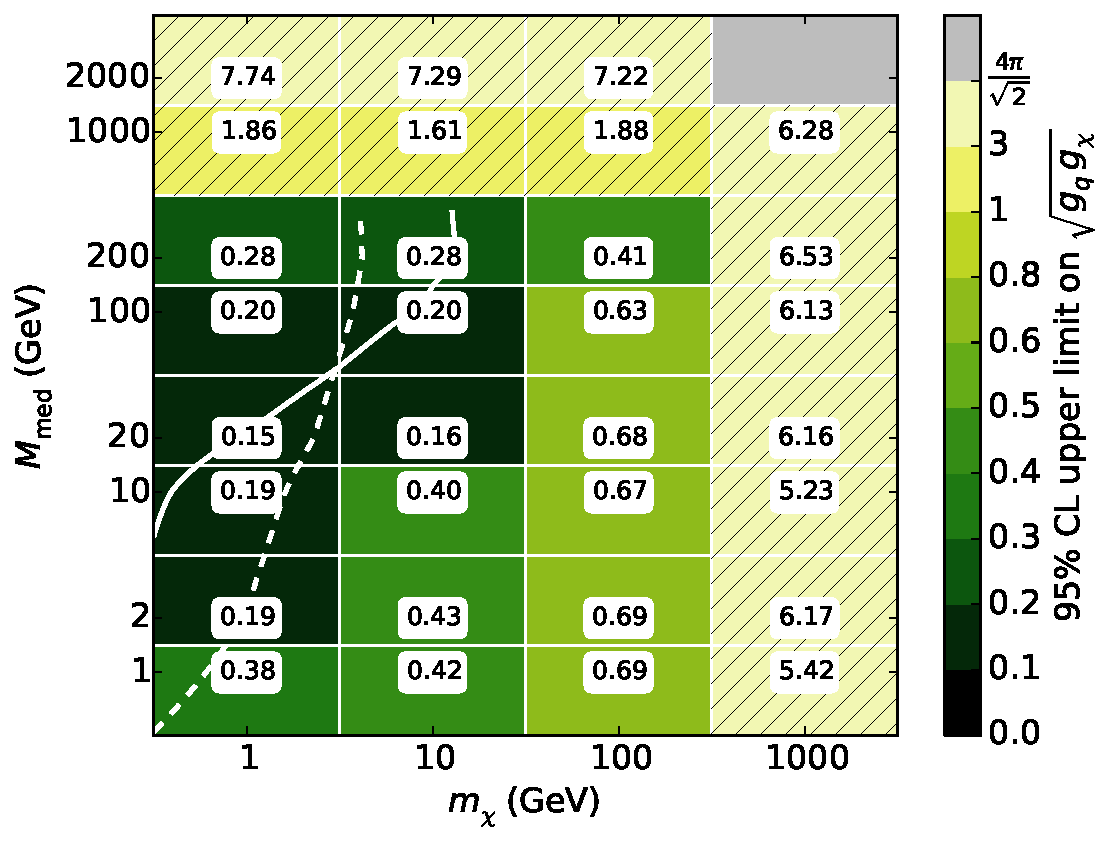
\includegraphics[width=1.\textwidth]{figures/grid_basepoints_SVD_rat05_monojet.pdf}
    \caption{sV model, $g_q/g_{\chi} = 0.5$, \monojet channel.}
  \end{subfigure}
  \begin{subfigure}[t]{0.32\textwidth}
    \centering
    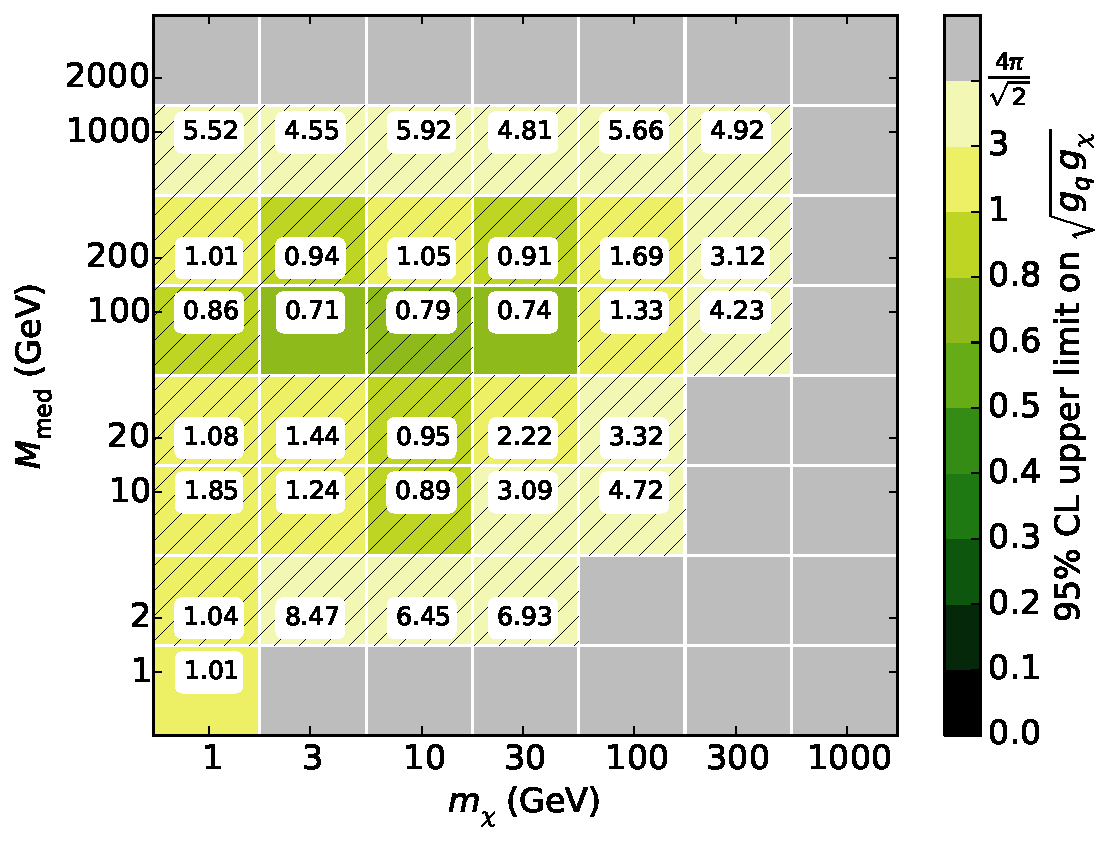
\includegraphics[width=1.\textwidth]{figures/grid_allpoints_SVD_rat05.pdf}
    \caption{sV model, $g_q/g_{\chi} = 0.5$, \monoZ channel.}
  \end{subfigure}
  \begin{subfigure}[t]{0.32\textwidth}
    \centering
    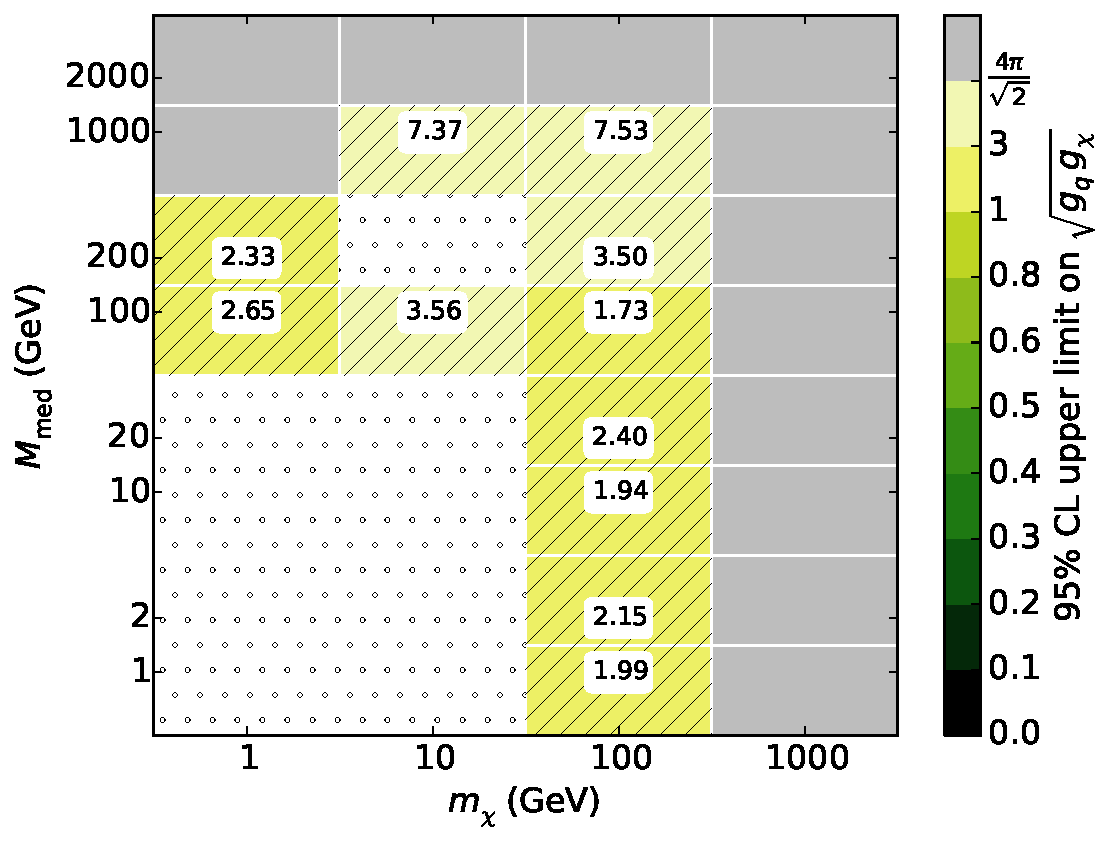
\includegraphics[width=1.\textwidth]{figures/grid_basepoints_SVD_rat05_monoWZ.pdf}
    \caption{sV model, $g_q/g_{\chi} = 0.5$, \monoWZ channel.}
    \vspace{0.75cm}
  \end{subfigure}
  \begin{subfigure}[t]{0.32\textwidth}
    \centering
    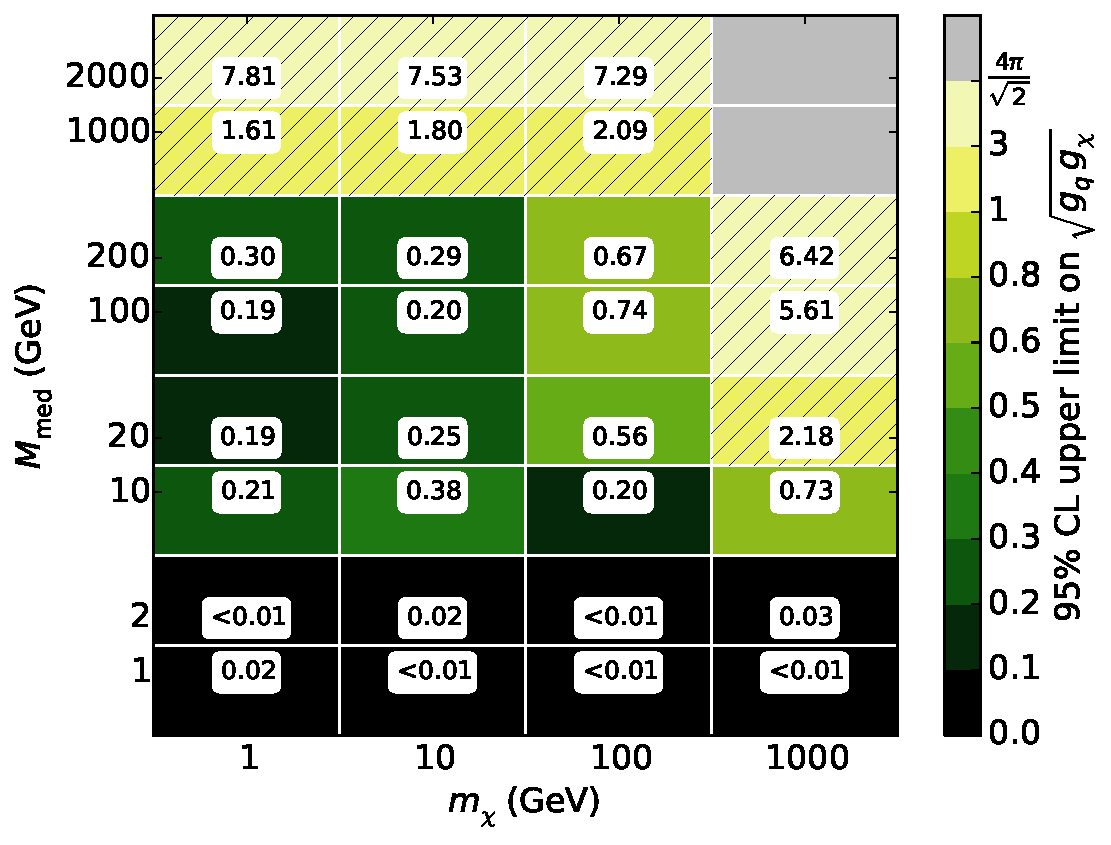
\includegraphics[width=1.\textwidth]{figures/grid_basepoints_SAD_rat05_monojet.pdf}
    \caption{sA model, $g_q/g_{\chi} = 0.5$, \monojet channel.}
  \end{subfigure}
  \begin{subfigure}[t]{0.32\textwidth}
    \centering
    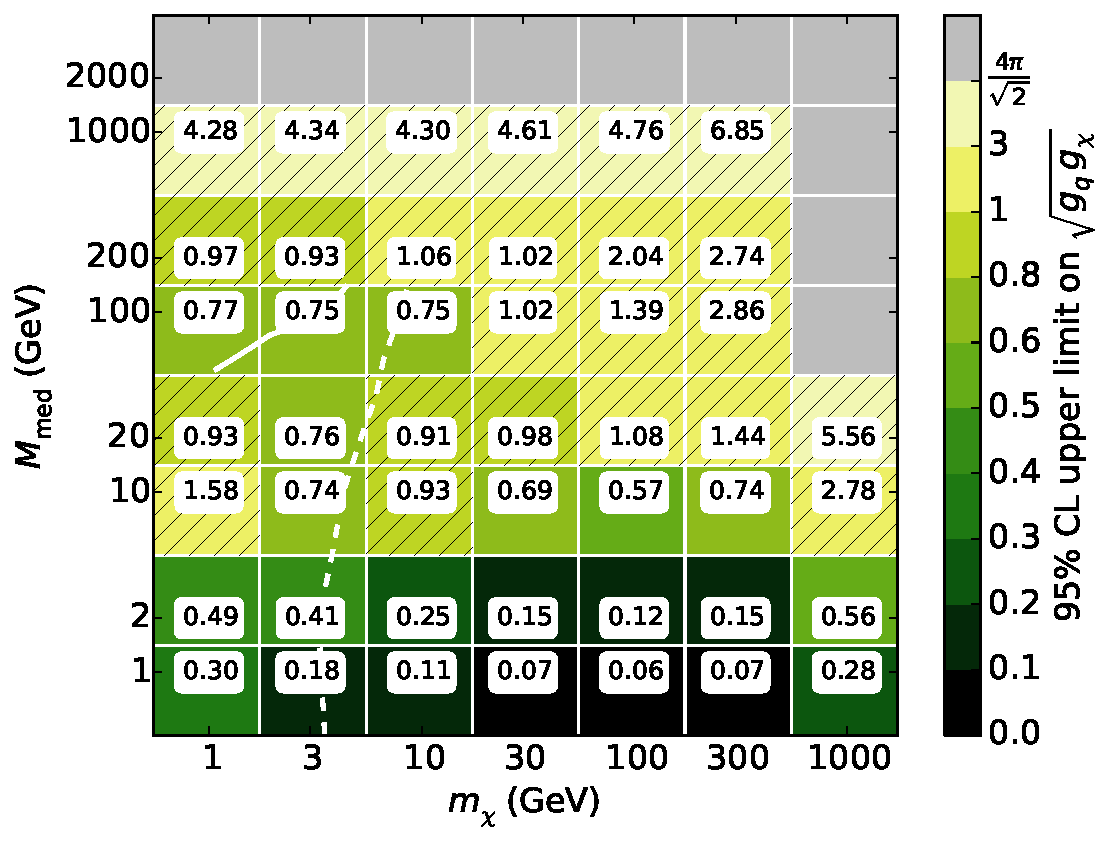
\includegraphics[width=1.\textwidth]{figures/grid_allpoints_SAD_rat05.pdf}
    \caption{sA model, $g_q/g_{\chi} = 0.5$, \monoZ channel.}
  \end{subfigure}
  \begin{subfigure}[t]{0.32\textwidth}
    \centering
    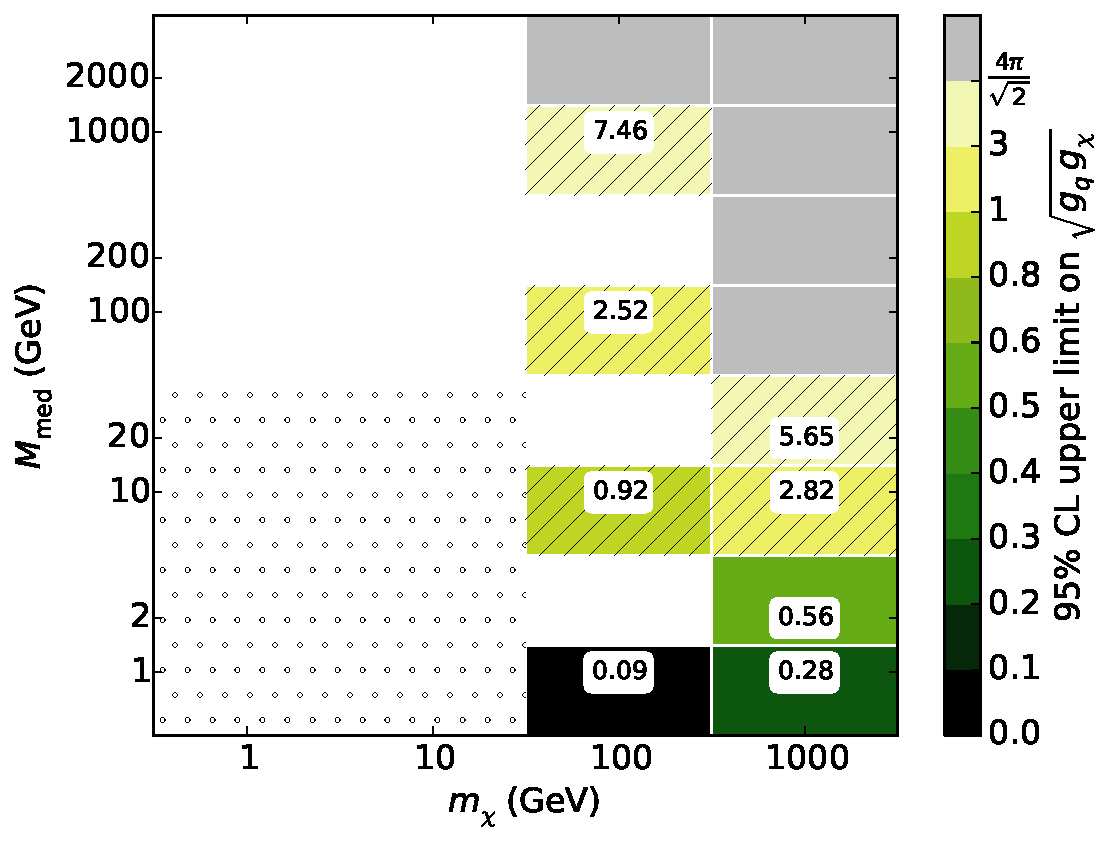
\includegraphics[width=1.\textwidth]{figures/grid_basepoints_SAD_rat05_monoWZ.pdf}
    \caption{sA model, $g_q/g_{\chi} = 0.5$, \monoWZ channel.}
  \end{subfigure}
  \caption{Upper limits on the coupling for the $s$-channel models in the \monojet (left), \monoZ (centre) and \monoWZ (right) channels, for $\gX / \gq$ = 0.5. The grey region represents the phase space where no meaningful limit was obtained. The hatched region represents a limit which leads to a width greater than $\Mmed / 2$, so the validity of the calculation begins to fail. The dotted region represents phase space where insufficient statistics were available.}
  \label{fig:results_sVsA_rat05}
\end{sidewaysfigure}

\begin{sidewaysfigure}
  \centering
  \begin{subfigure}[t]{0.32\textwidth}
    \centering
    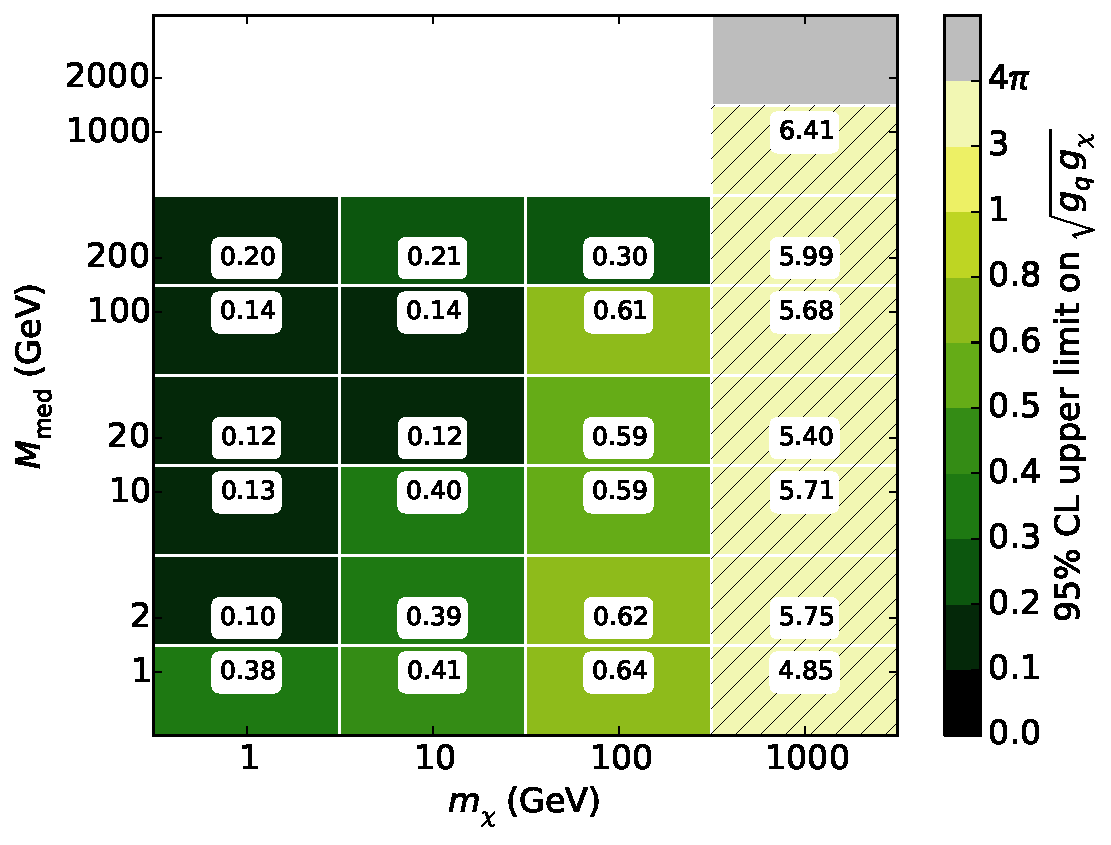
\includegraphics[width=1.\textwidth]{figures/grid_basepoints_SVD_rat1_monojet.pdf}
    \caption{sV model, $g_q/g_{\chi} = 1$, \monojet channel.}
  \end{subfigure}
  \begin{subfigure}[t]{0.32\textwidth}
    \centering
    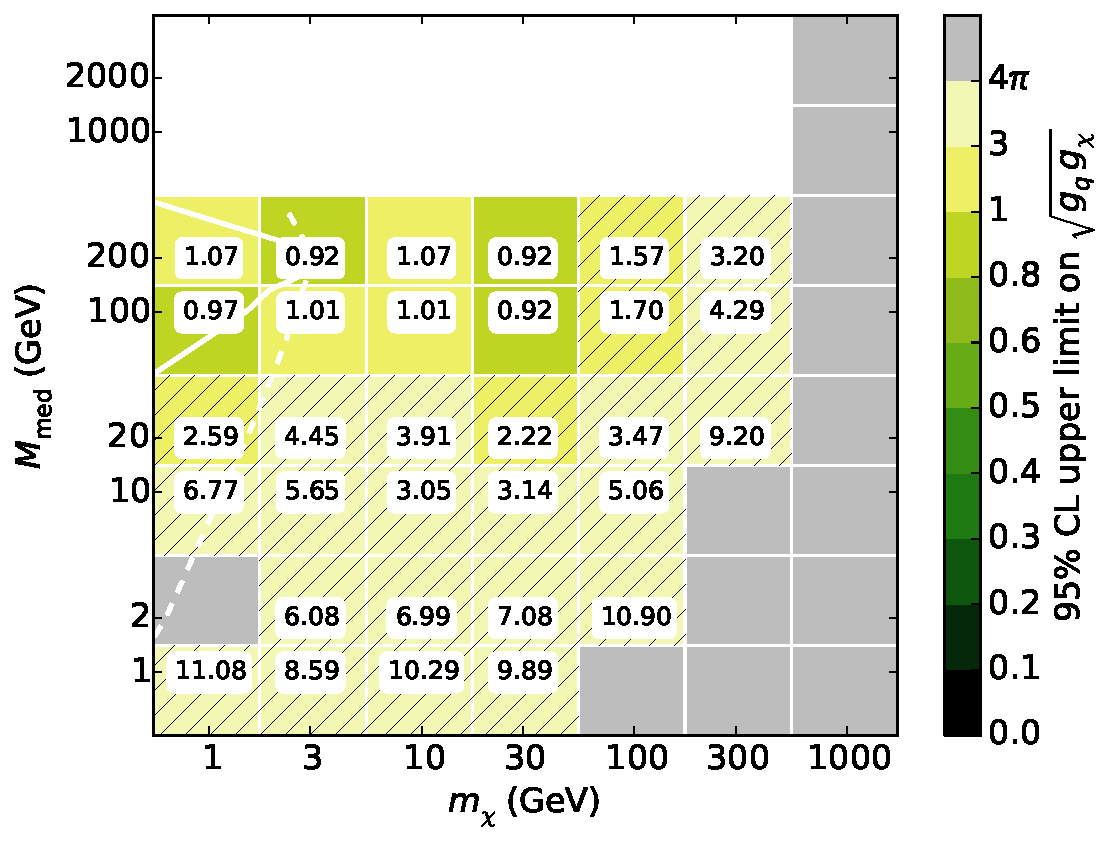
\includegraphics[width=1.\textwidth]{figures/grid_allpoints_SVD_rat1.pdf}
    \caption{sV model, $g_q/g_{\chi} = 1$, \monoZ channel.}
  \end{subfigure}
  \begin{subfigure}[t]{0.32\textwidth}
    \centering
    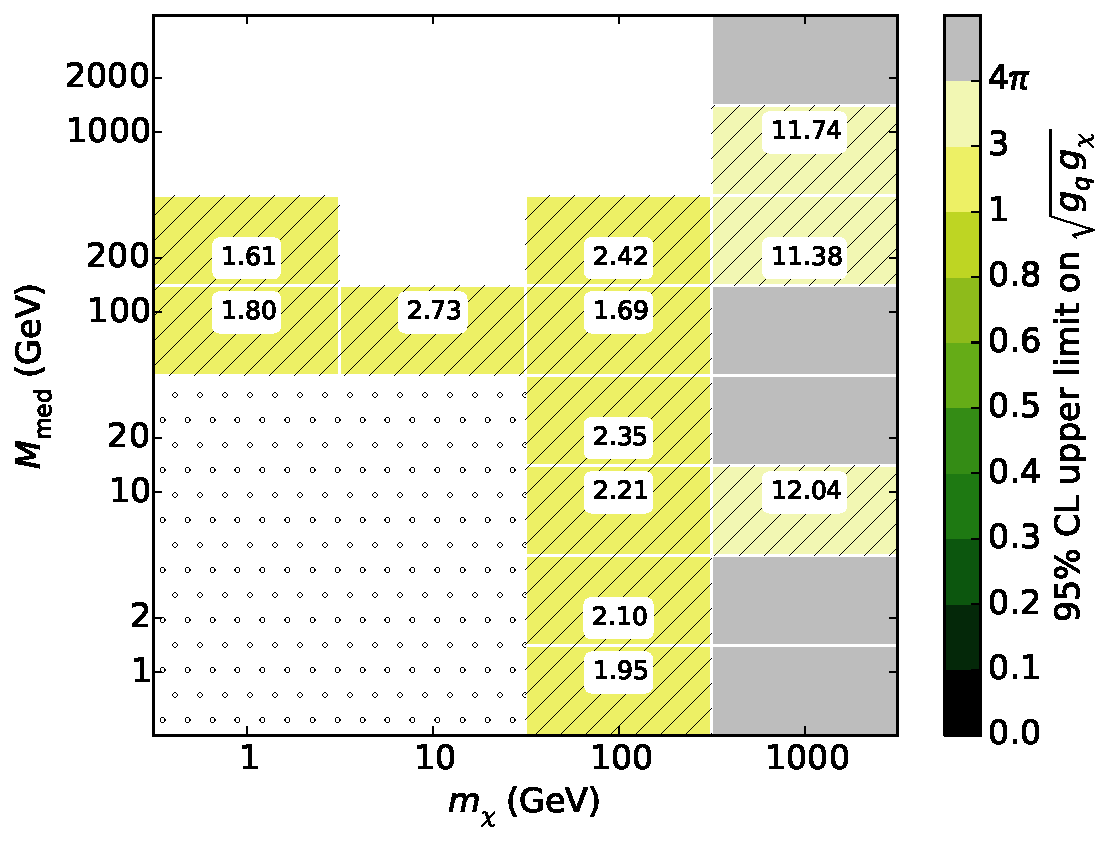
\includegraphics[width=1.\textwidth]{figures/grid_basepoints_SVD_rat1_monoWZ.pdf}
    \caption{sV model, $g_q/g_{\chi} = 1$, \monoWZ channel.}
    \vspace{0.75cm}
  \end{subfigure}
  \begin{subfigure}[t]{0.32\textwidth}
    \centering
    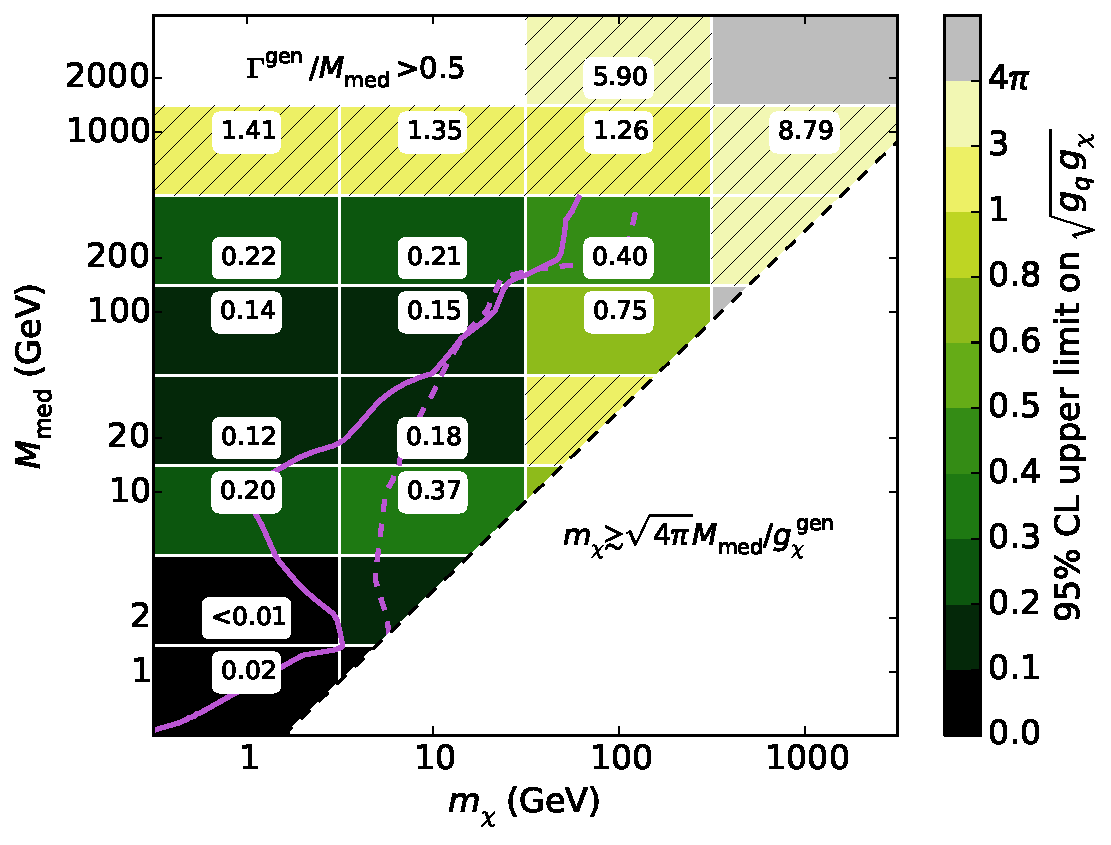
\includegraphics[width=1.\textwidth]{figures/grid_basepoints_SAD_rat1_monojet.pdf}
    \caption{sA model, $g_q/g_{\chi} = 1$, \monojet channel.}
  \end{subfigure}
  \begin{subfigure}[t]{0.32\textwidth}
    \centering
    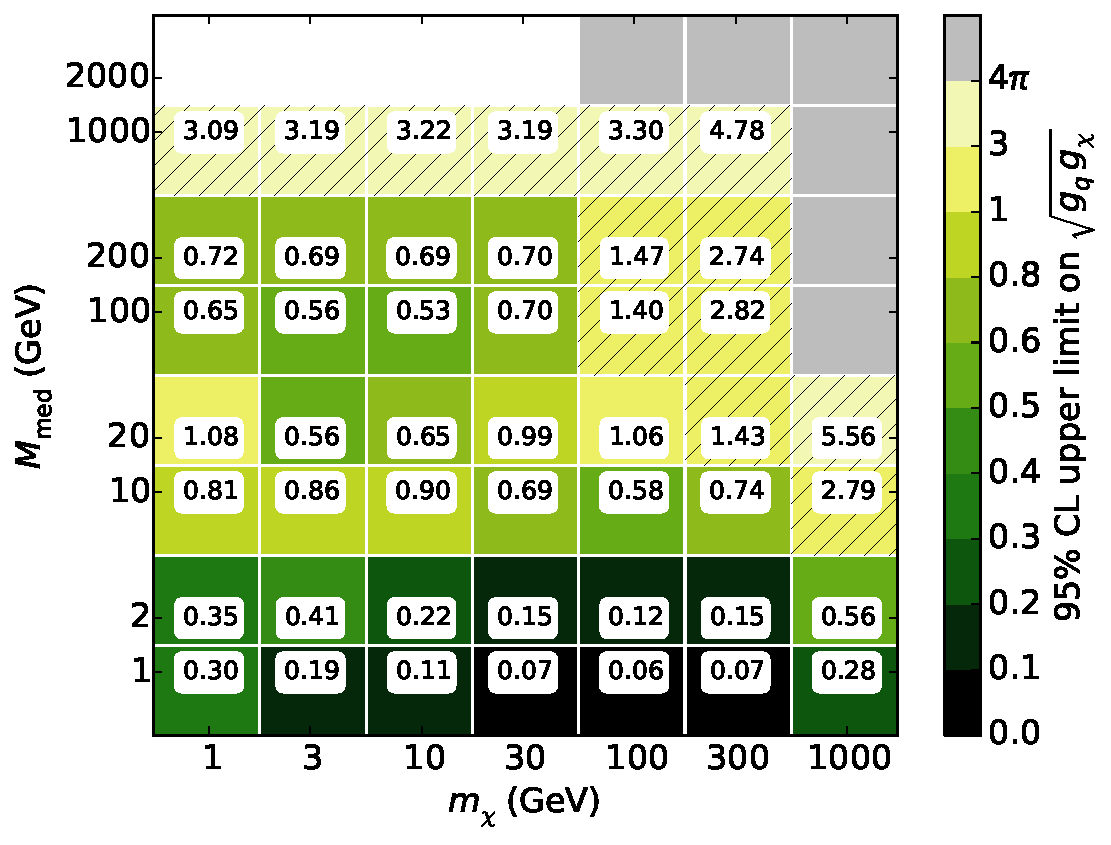
\includegraphics[width=1.\textwidth]{figures/grid_allpoints_SAD_rat1.pdf}
    \caption{sA model, $g_q/g_{\chi} = 1$, \monoZ channel.}
  \end{subfigure}
  \begin{subfigure}[t]{0.32\textwidth}
    \centering
    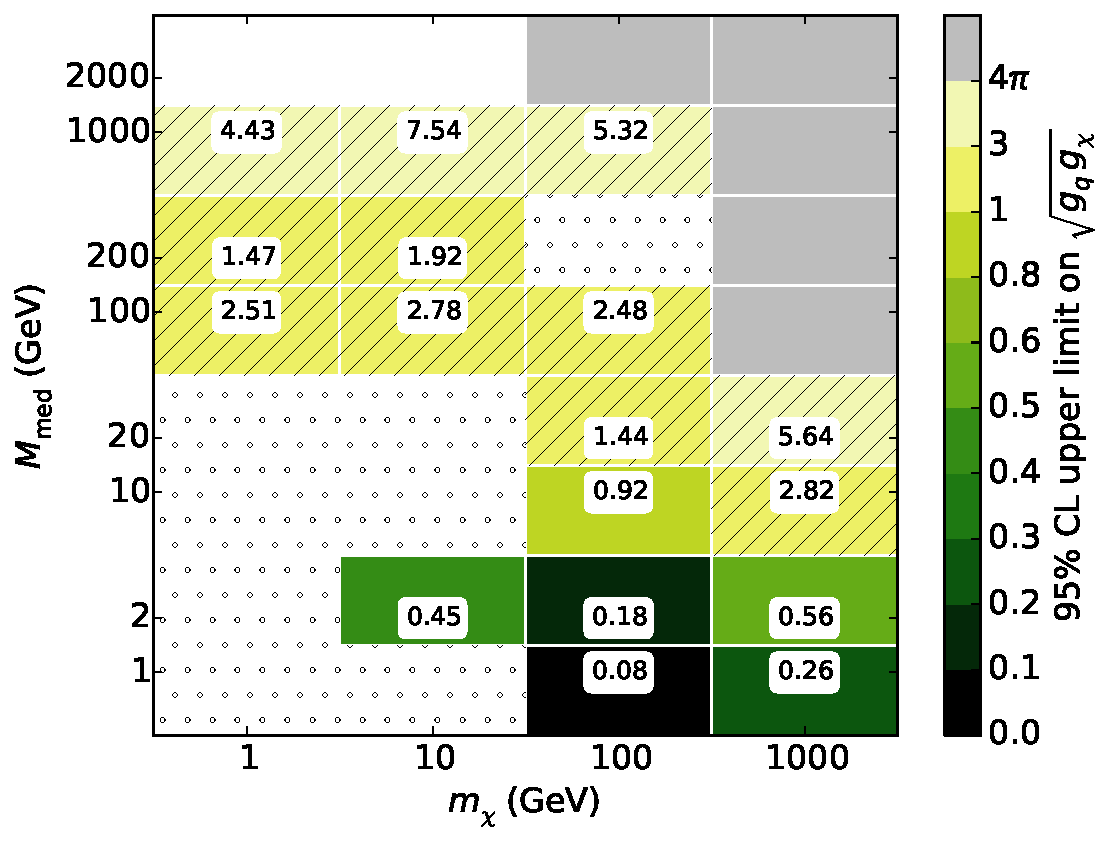
\includegraphics[width=1.\textwidth]{figures/grid_basepoints_SAD_rat1_monoWZ.pdf}
    \caption{sA model, $g_q/g_{\chi} = 1$, \monoWZ channel.}
  \end{subfigure}
  \caption{Upper limits on the couplings for the $s$-channel models in the \monojet (left), \monoZ (centre) and \monoWZ (right) channels, for $\gX / \gq$ = 1. Refer to fig.~\ref{fig:results_sVsA_rat05} for details.}
  \label{fig:results_sVsA_rat1}
\end{sidewaysfigure}

\begin{sidewaysfigure}
  \centering
  \begin{subfigure}[t]{0.32\textwidth}
    \centering
    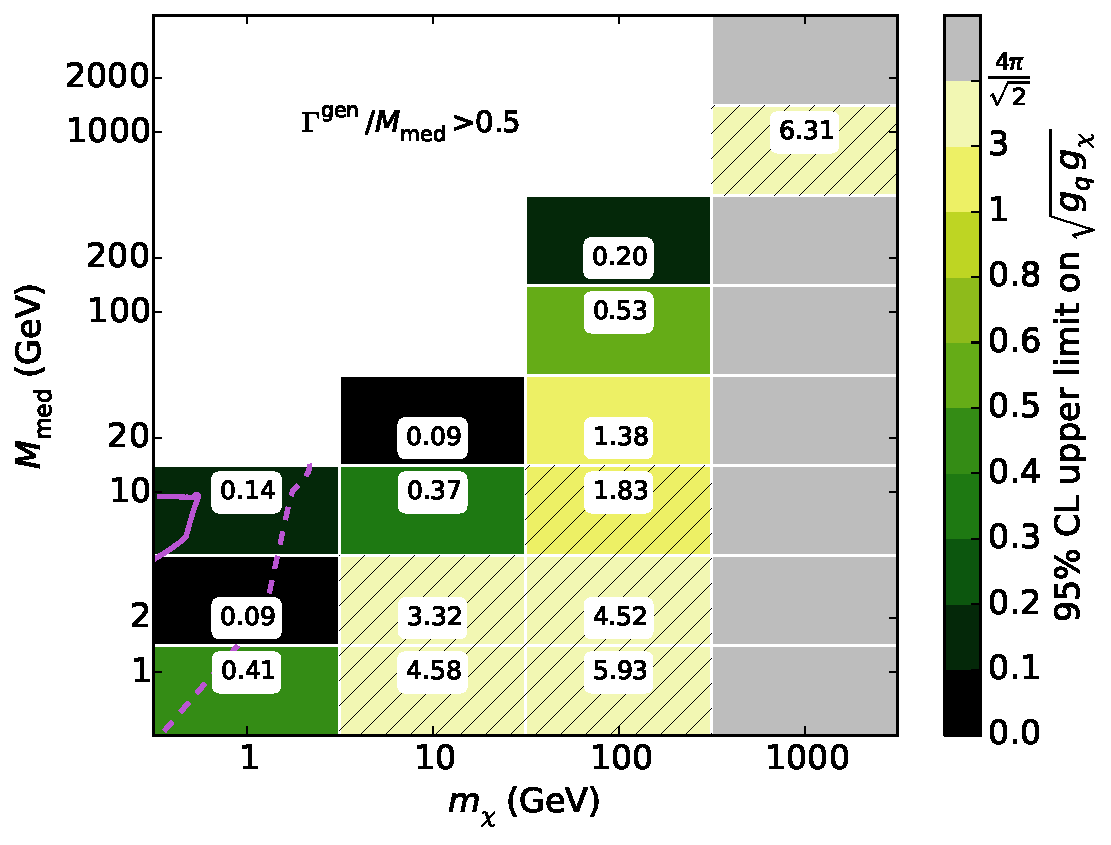
\includegraphics[width=1.\textwidth]{figures/grid_basepoints_SVD_rat2_monojet.pdf}
    \caption{sV model, $g_q/g_{\chi} = 2$, \monojet channel.}
  \end{subfigure}
  \begin{subfigure}[t]{0.32\textwidth}
    \centering
    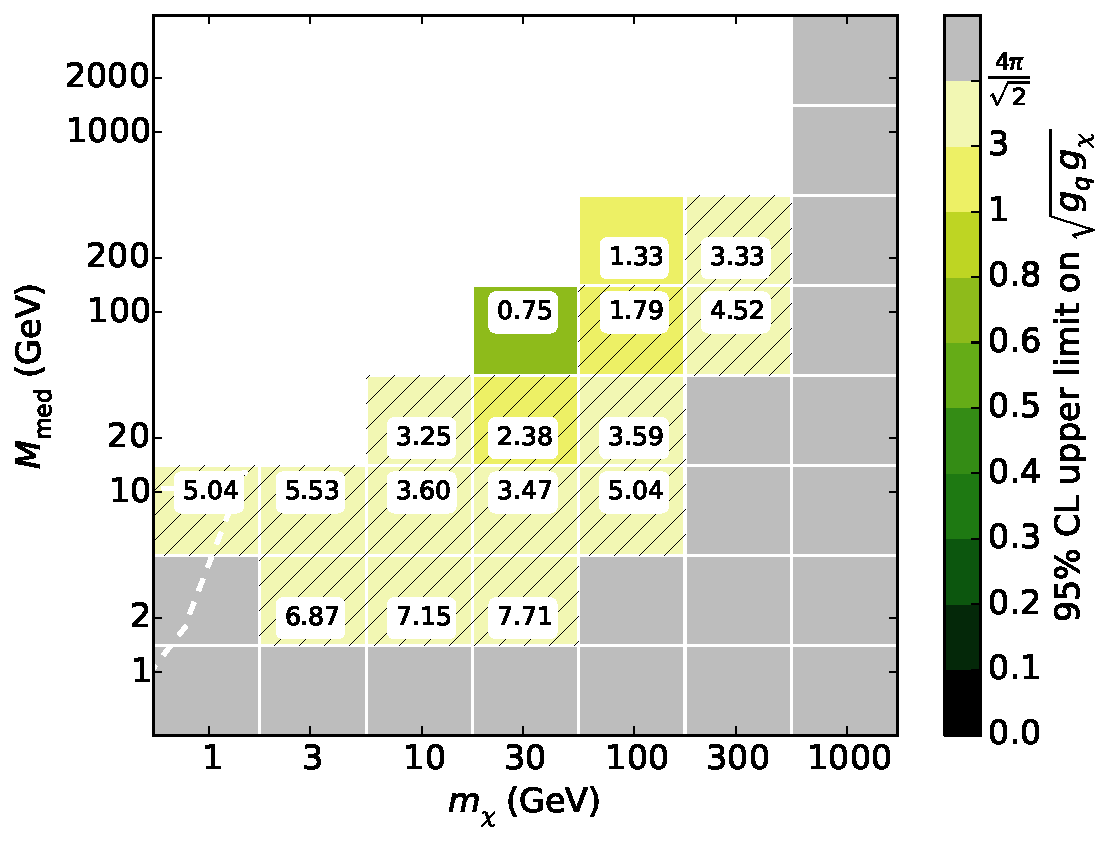
\includegraphics[width=1.\textwidth]{figures/grid_allpoints_SVD_rat2.pdf}
    \caption{sV model, $g_q/g_{\chi} = 2$, \monoZ channel.}
  \end{subfigure}
  \begin{subfigure}[t]{0.32\textwidth}
    \centering
    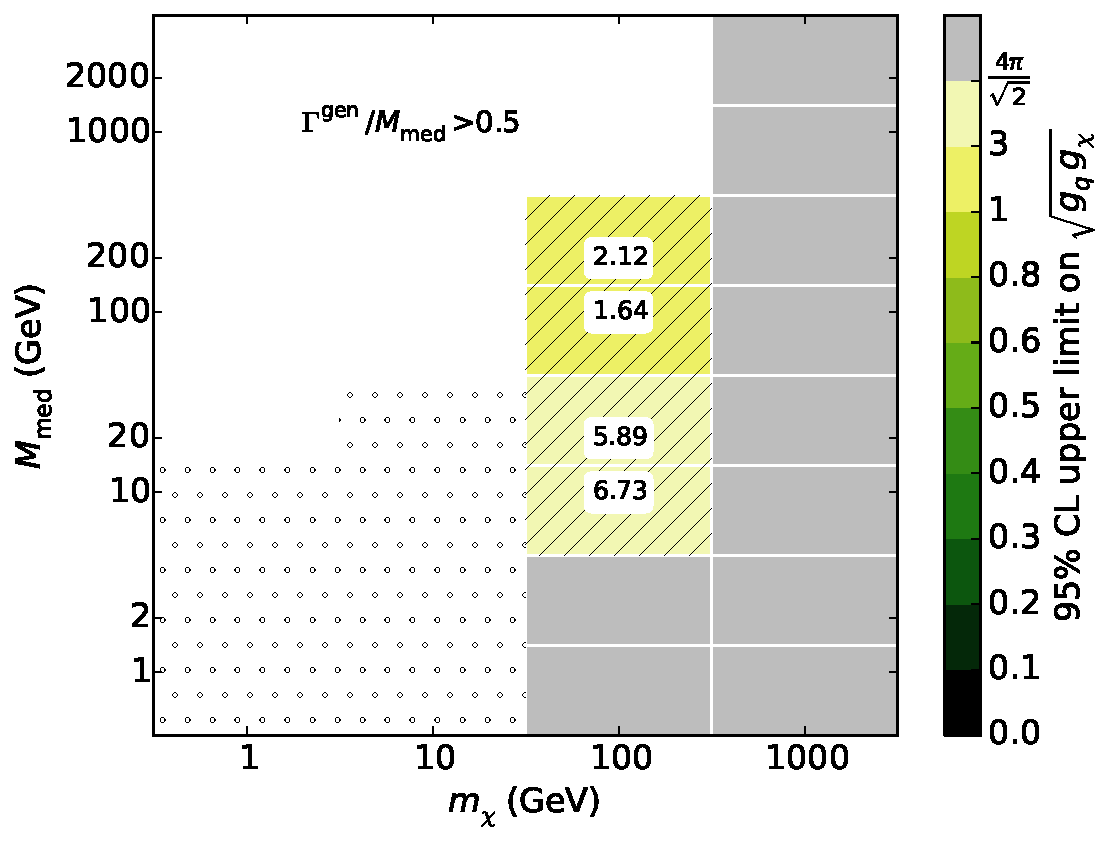
\includegraphics[width=1.\textwidth]{figures/grid_basepoints_SVD_rat2_monoWZ.pdf}
    \caption{sV model, $g_q/g_{\chi} = 2$, \monoWZ channel.}
    \vspace{0.75cm}
  \end{subfigure}
  \begin{subfigure}[t]{0.32\textwidth}
    \centering
    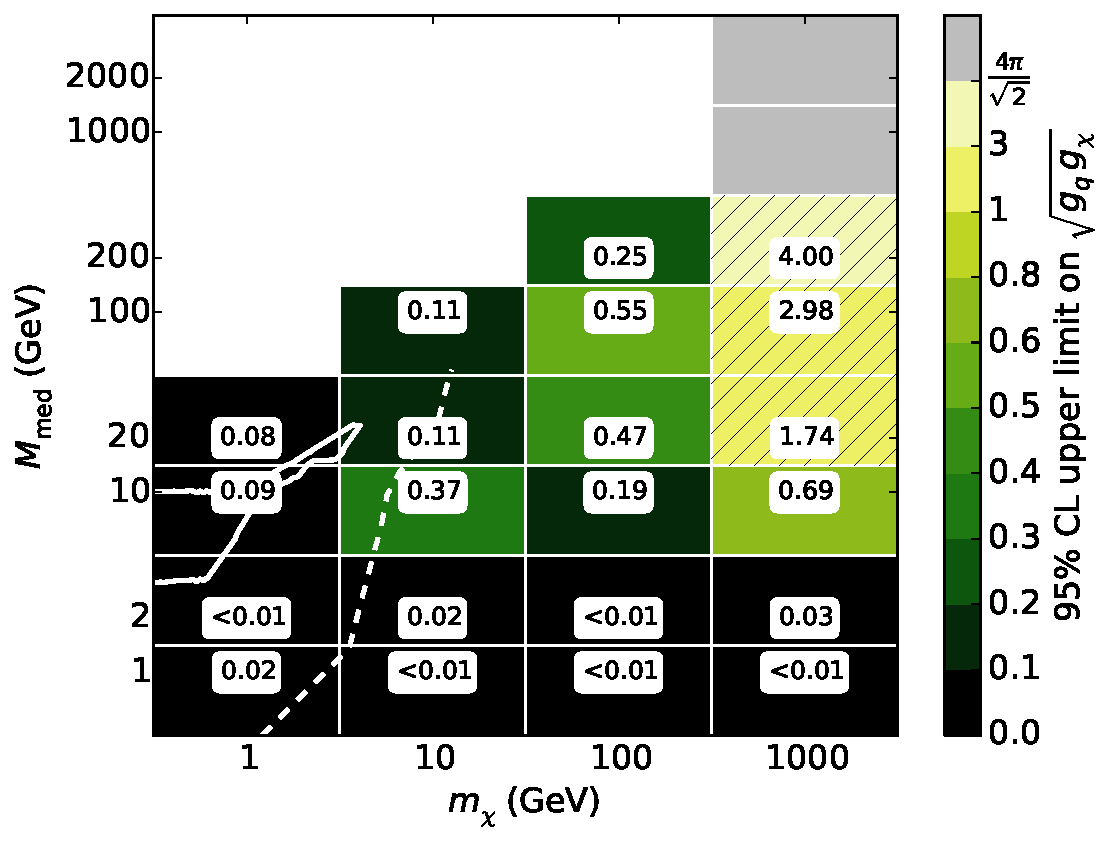
\includegraphics[width=1.\textwidth]{figures/grid_basepoints_SAD_rat2_monojet.pdf}
    \caption{sA model, $g_q/g_{\chi} = 2$, \monojet channel.}
  \end{subfigure}
  \begin{subfigure}[t]{0.32\textwidth}
    \centering
    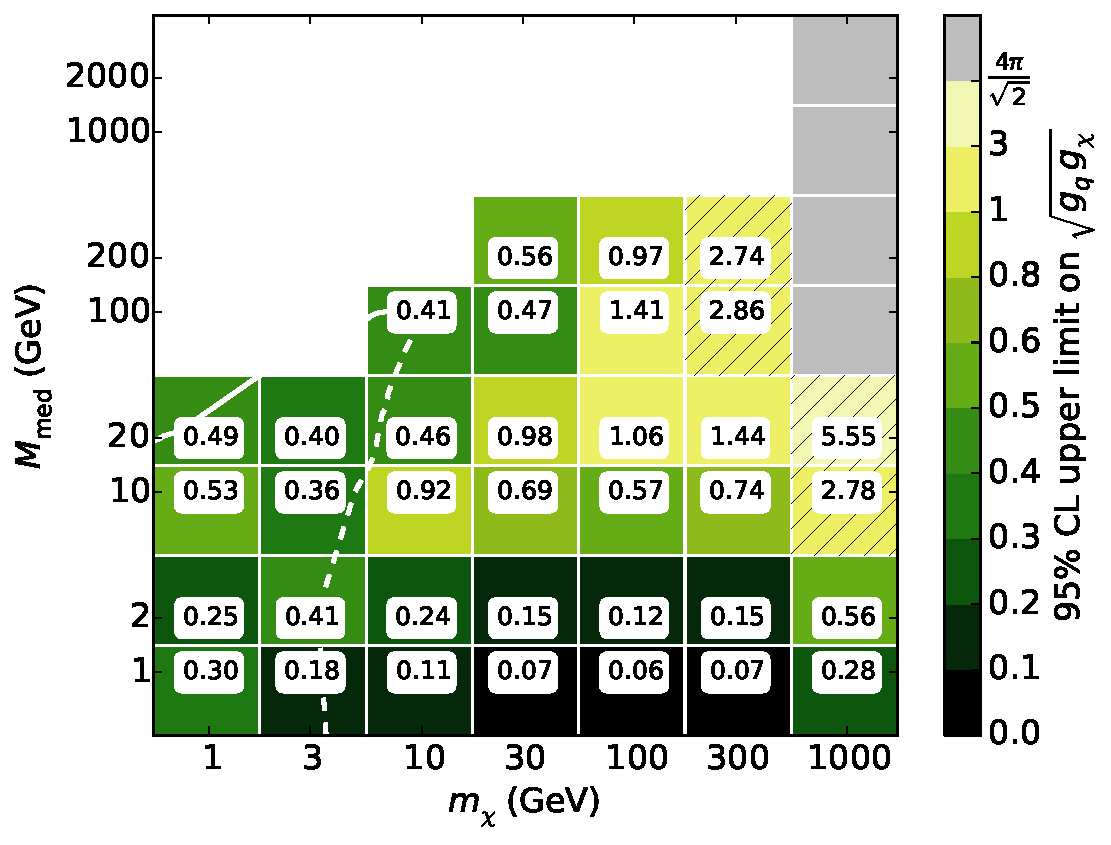
\includegraphics[width=1.\textwidth]{figures/grid_allpoints_SAD_rat2.pdf}
    \caption{sA model, $g_q/g_{\chi} = 2$, \monoZ channel.}
  \end{subfigure}
  \begin{subfigure}[t]{0.32\textwidth}
    \centering
    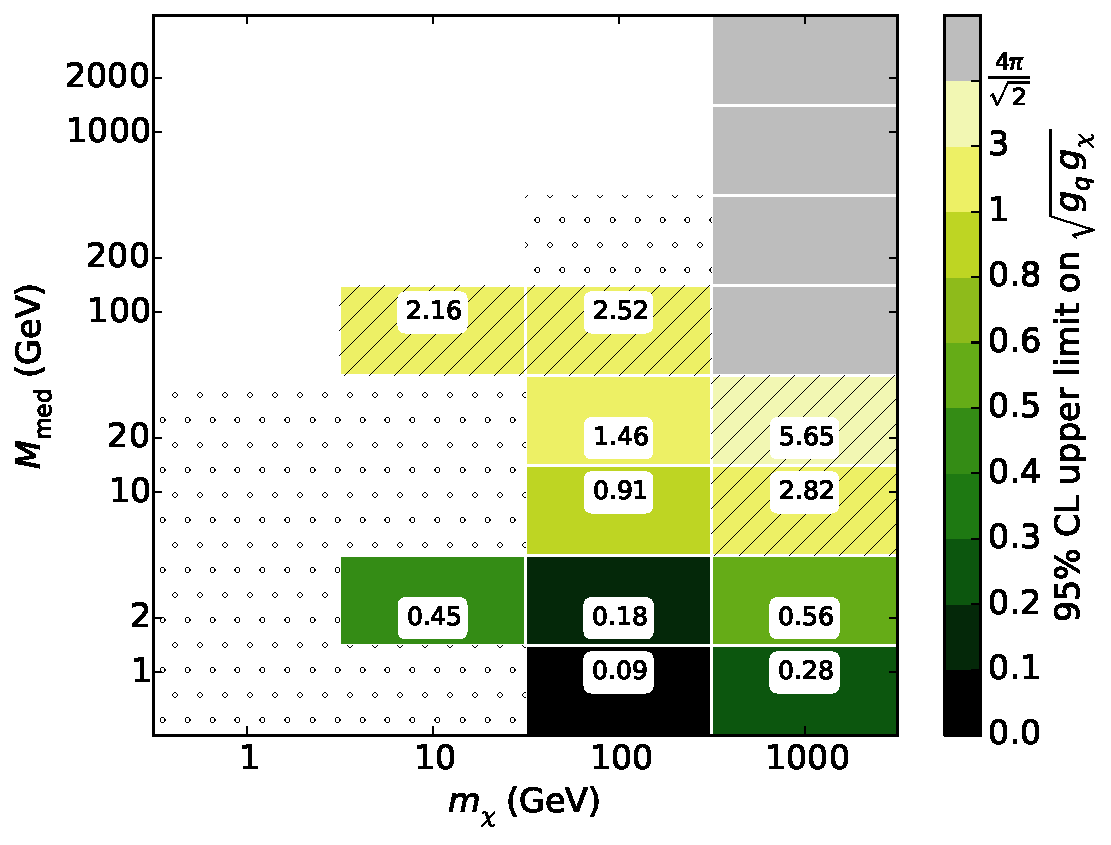
\includegraphics[width=1.\textwidth]{figures/grid_basepoints_SAD_rat2_monoWZ.pdf}
    \caption{sA model, $g_q/g_{\chi} = 2$, \monoWZ channel.}
  \end{subfigure}
  \caption{Upper limits on the coupling for the $s$-channel models in the \monojet (left), \monoZ (centre) and \monoWZ (right) channels, for $\gX / \gq$ = 2. Refer to fig.~\ref{fig:results_sVsA_rat05} for details.}
  \label{fig:results_sVsA_rat2}
\end{sidewaysfigure}

\begin{sidewaysfigure}
  \centering
  \begin{subfigure}[t]{0.32\textwidth}
    \centering
    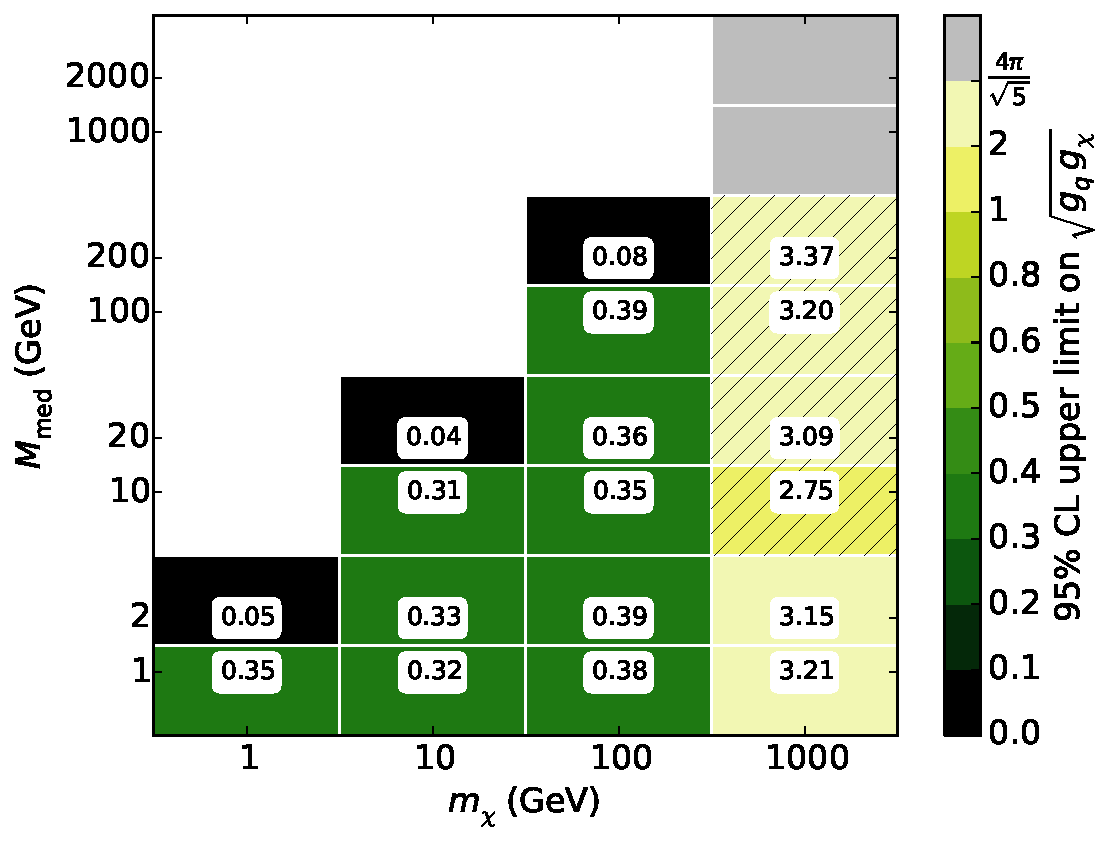
\includegraphics[width=1.\textwidth]{figures/grid_basepoints_SVD_rat5_monojet.pdf}
    \caption{sV model, $g_q/g_{\chi} = 5$, \monojet channel.}
  \end{subfigure}
  \begin{subfigure}[t]{0.32\textwidth}
    \centering
    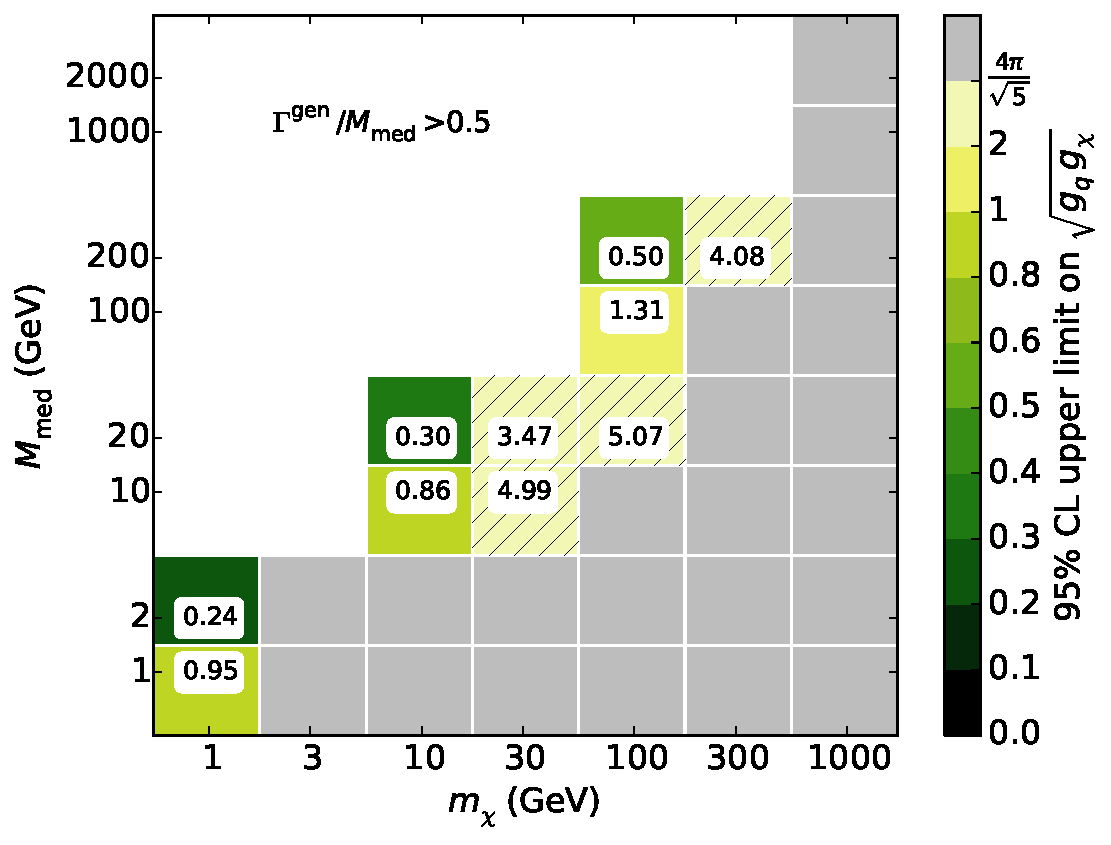
\includegraphics[width=1.\textwidth]{figures/grid_allpoints_SVD_rat5.pdf}
    \caption{sV model, $g_q/g_{\chi} = 5$, \monoZ channel.}
  \end{subfigure}
  \begin{subfigure}[t]{0.32\textwidth}
    \centering
    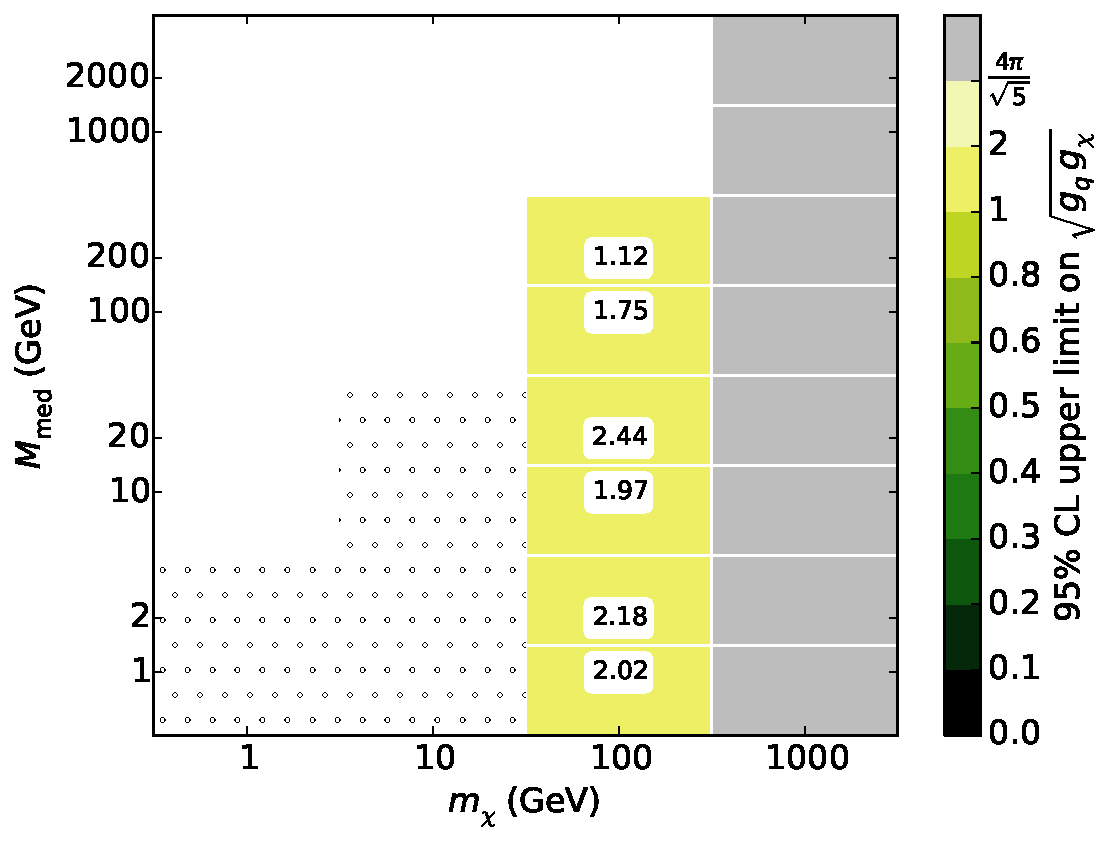
\includegraphics[width=1.\textwidth]{figures/grid_basepoints_SVD_rat5_monoWZ.pdf}
    \caption{sV model, $g_q/g_{\chi} = 5$, \monoWZ channel.}
    \vspace{0.75cm}
  \end{subfigure}
  \begin{subfigure}[t]{0.32\textwidth}
    \centering
    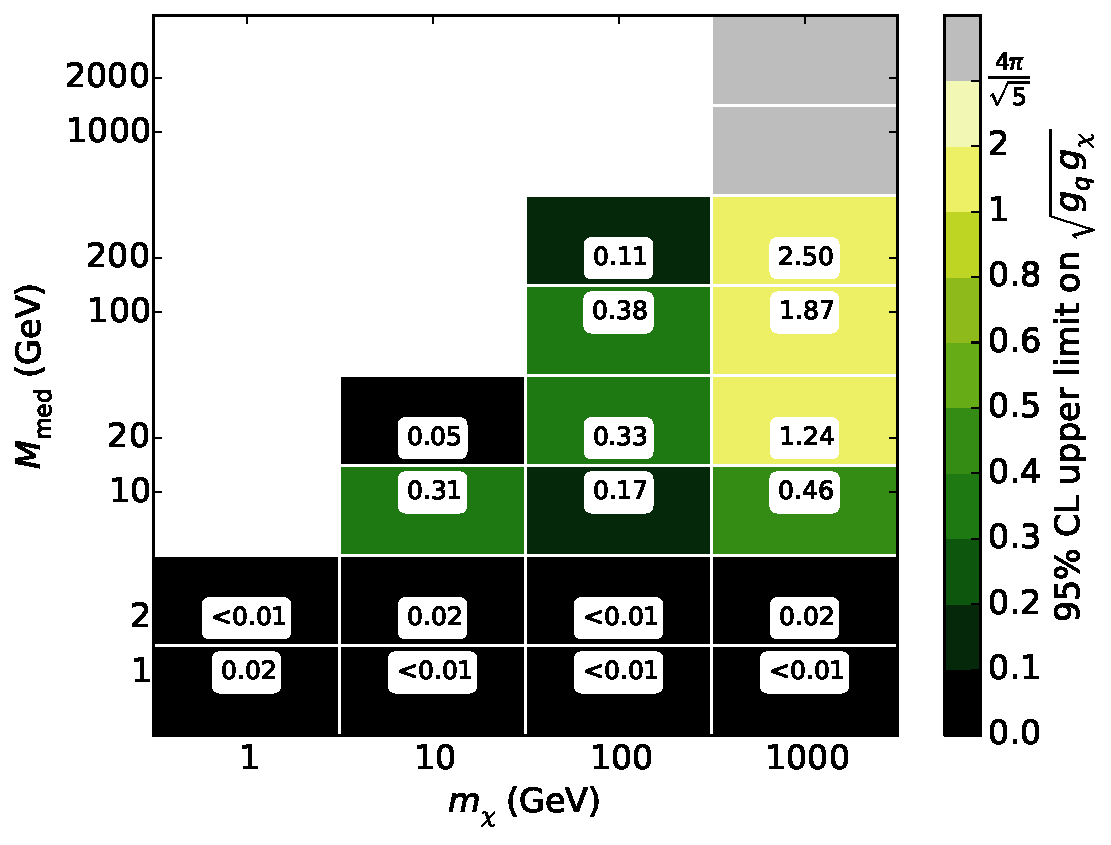
\includegraphics[width=1.\textwidth]{figures/grid_basepoints_SAD_rat5_monojet.pdf}
    \caption{sA model, $g_q/g_{\chi} = 5$, \monojet channel.}
  \end{subfigure}
  \begin{subfigure}[t]{0.32\textwidth}
    \centering
    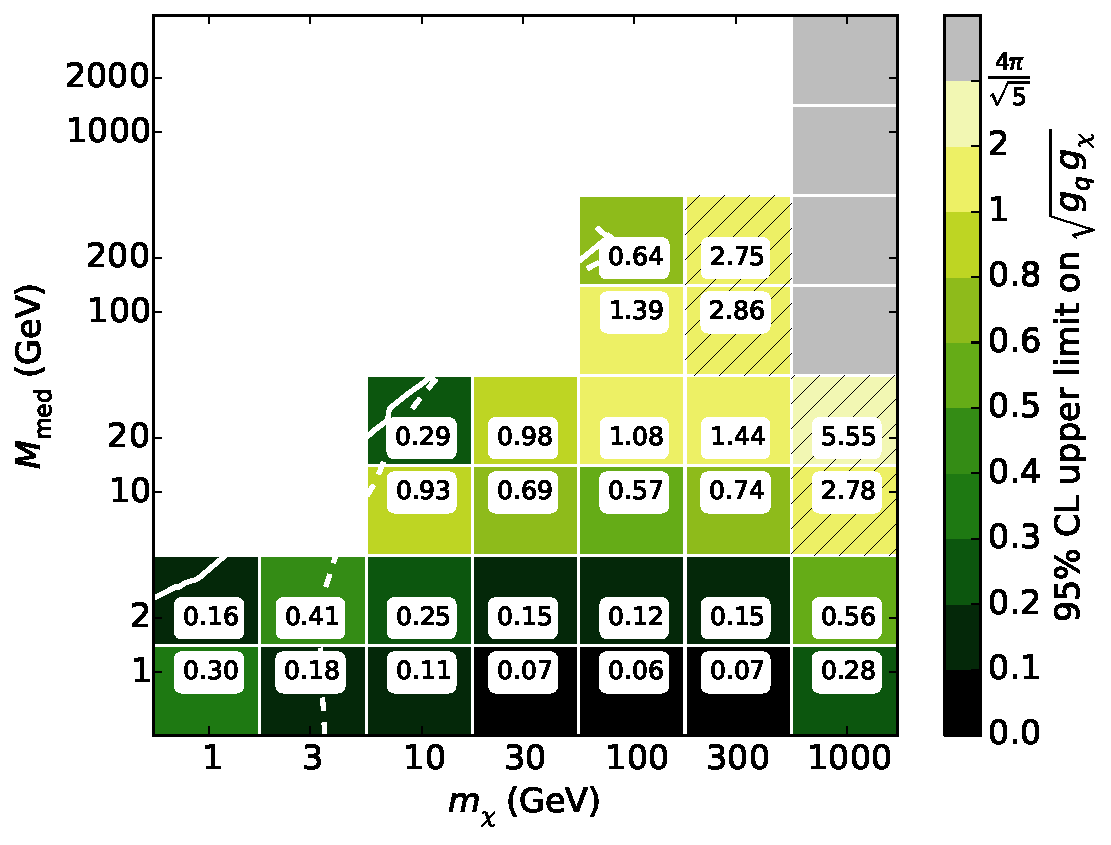
\includegraphics[width=1.\textwidth]{figures/grid_allpoints_SAD_rat5.pdf}
    \caption{sA model, $g_q/g_{\chi} = 5$, \monoZ channel.}
  \end{subfigure}
  \begin{subfigure}[t]{0.32\textwidth}
    \centering
    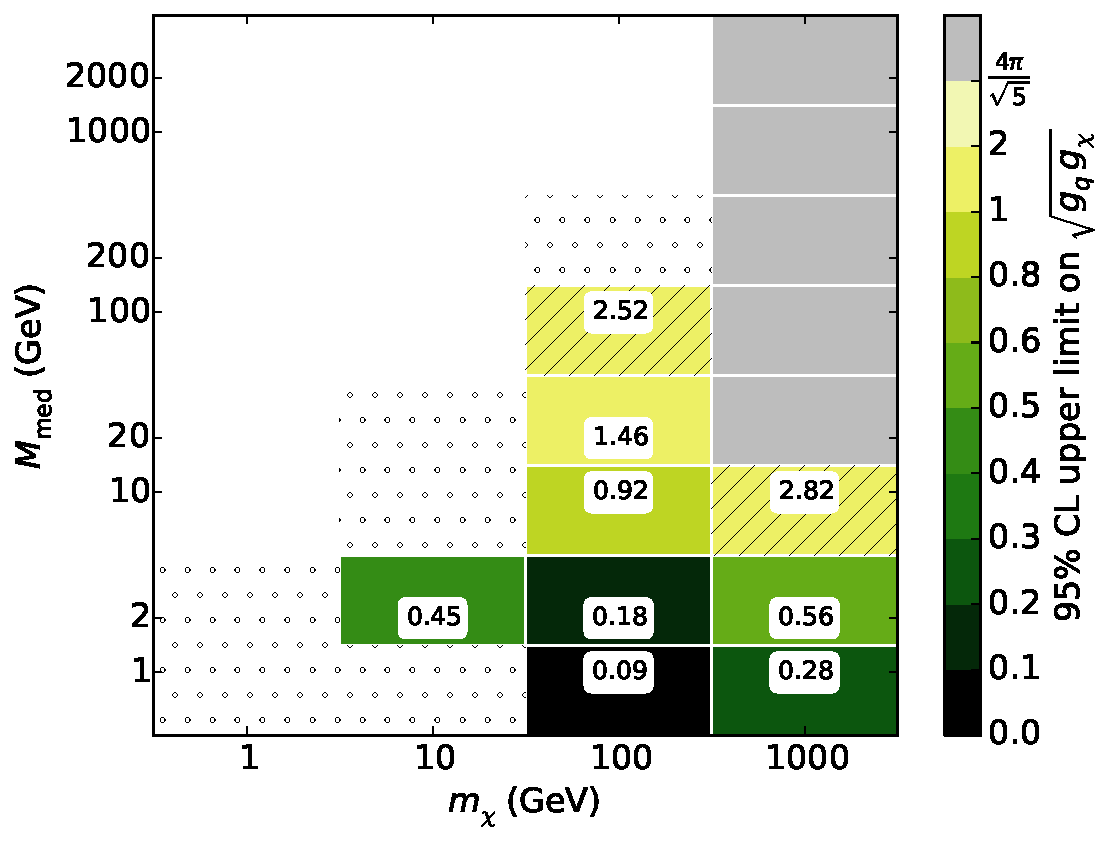
\includegraphics[width=1.\textwidth]{figures/grid_basepoints_SAD_rat5_monoWZ.pdf}
    \caption{sA model, $g_q/g_{\chi} = 5$, \monoWZ channel.}
  \end{subfigure}
  \caption{Upper limits on the coupling for the $s$-channel models in the \monojet (left), \monoZ (centre) and \monoWZ (right) channels, for $\gX / \gq$ = 5. Refer to fig.~\ref{fig:results_sVsA_rat05} for details.}
  \label{fig:results_sVsA_rat5}
\end{sidewaysfigure}

\begin{figure}
  \centering
  \begin{subfigure}[t]{0.495\textwidth}
    \centering
    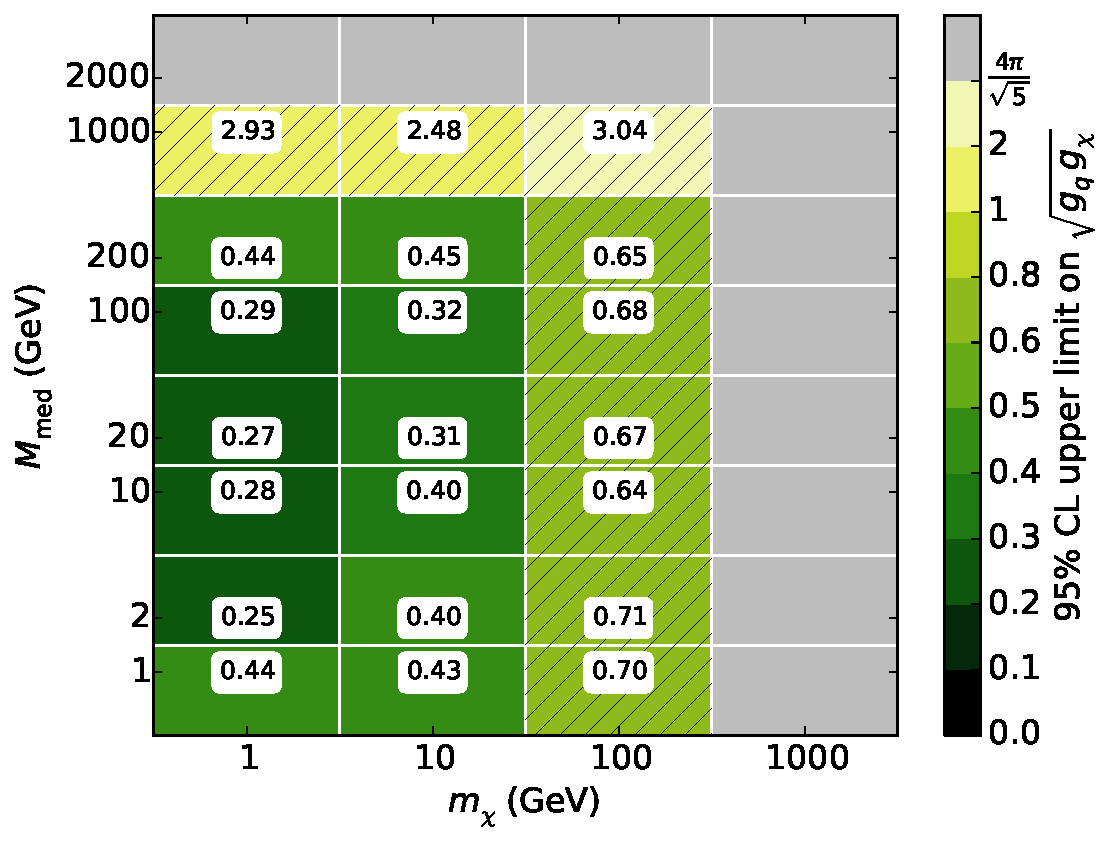
\includegraphics[width=1.\textwidth]{figures/grid_basepoints_SVD_rat02_monojet.pdf}
    \caption{sV model, $g_q/g_{\chi} = 0.2$, \monojet channel.}
  \end{subfigure}
  \begin{subfigure}[t]{0.495\textwidth}
    \centering
    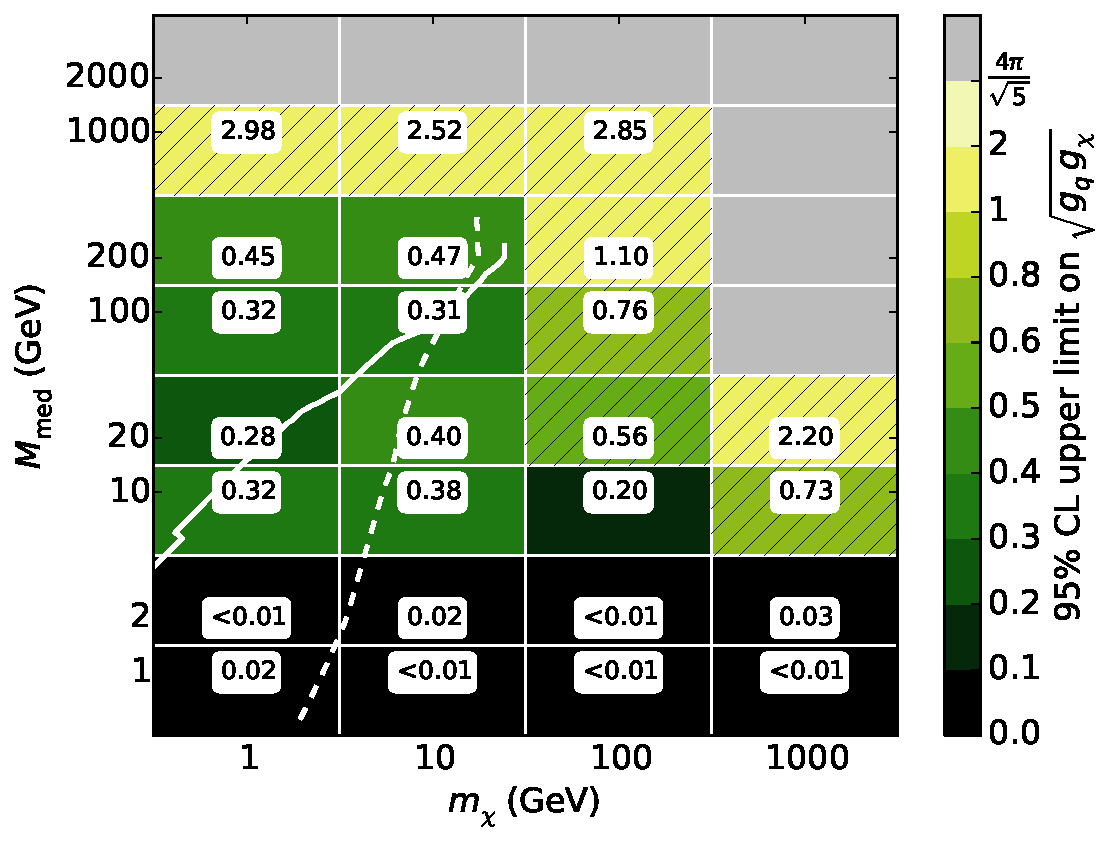
\includegraphics[width=1.\textwidth]{figures/grid_basepoints_SAD_rat02_monojet.pdf}
    \caption{sA model, $g_q/g_{\chi} = 0.2$, \monojet channel.}
  \end{subfigure}
  \caption{Upper limits on the coupling for the $s$-channel models in the \monojet channel, for $\gX / \gq$ = 0.2. Refer to fig.~\ref{fig:results_sVsA_rat05} for details.}
  \label{fig:results_sVsA_rat02}
\end{figure}

\begin{figure}
  \centering
  \begin{subfigure}[t]{0.495\textwidth}
    \centering
    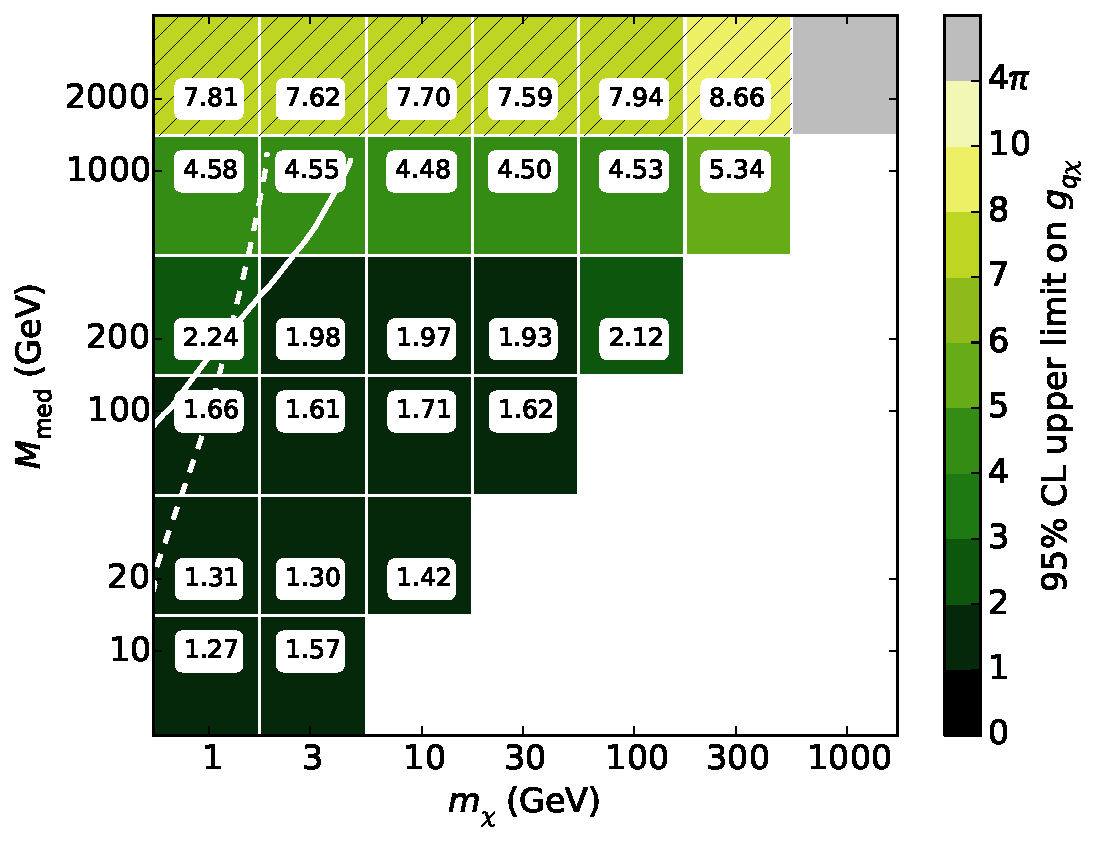
\includegraphics[width=1.\textwidth]{figures/grid_allpoints_TSD_rat1.pdf}
    \caption{tS model, \monoZ channel.}
  \end{subfigure}
  \begin{subfigure}[t]{0.495\textwidth}
    \centering
    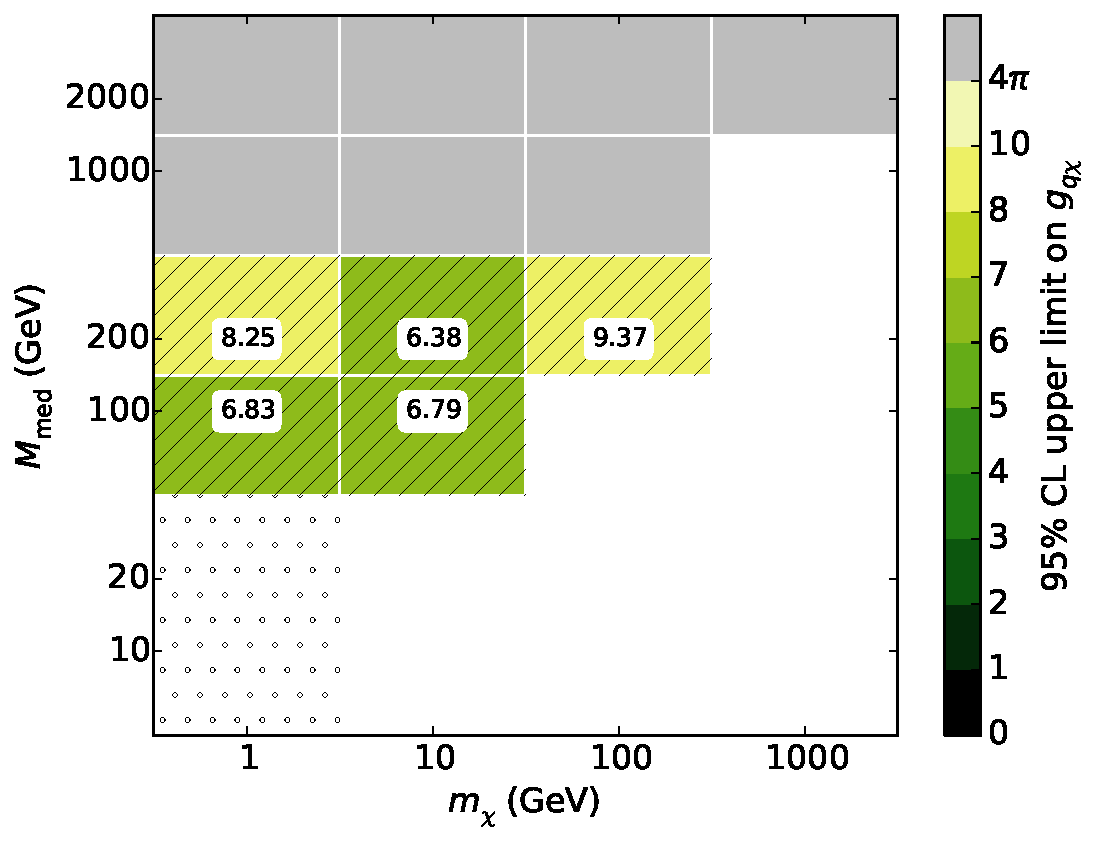
\includegraphics[width=1.\textwidth]{figures/grid_basepoints_TSD_rat1_monoWZ.pdf}
    \caption{tS model, \monoWZ channel.}
  \end{subfigure}
  \caption{Upper limits on the coupling $\gqX$ for the $t$-channel model in the \monoZ (left) and \monoWZ (right) channels. Refer to fig.~\ref{fig:results_sVsA_rat05} for details.}
  \label{fig:results_tS}
\end{figure}
